\documentclass[twoside,10pt]{report}
\usepackage{/Users/bradenhoagland/latex/styles/toggles}
\toggletrue{sectionbreaks}
%\toggletrue{sectionheaders}
\newcommand{\docTitle}{Category Theory}
\usepackage{/Users/bradenhoagland/latex/styles/common}
\importStyles{modern}{rainbow}{boxy}

\DeclareMathOperator{\op}{op}
\DeclareMathOperator{\ob}{ob}

\begin{document}
\tableofcontents

%+-------------------+
%| +---------------+ |
%| |    Chapter    | |
%| +---------------+ |
%+-------------------+
% The Basics

\chapter{The Basics}

%%%%%%%%%%%%%%%%%%%%
% Categories
%%%%%%%%%%%%%%%%%%%%

\section{Categories}


\begin{defn}
	A \textbf{category} $\cat{C}$ is a collection of \textbf{objects} $\ob(\cat{C})$ and \textbf{morphisms} $\mor({\cat{C} })$, where $\hom(A,B)$ denotes the morphsisms from object $A$ to object $B$. There are several requirements:
	\begin{enumerate}
		\item Morphisms must compose: $(f, g) \mapsto gf.$
		\item Morphism composition is associative.
		\item If $A \neq C$ or $B \neq D$, then $\hom(A,B)$ and $\hom(C,D)$ are disjoint.
		\item Each object has an identity morphism, which is a two-sided identity.
	\end{enumerate}
\end{defn}
\begin{figure}[H]
	\centering
	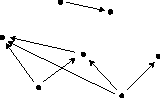
\includegraphics[scale=1.4]{fig/category.pdf}
\end{figure}

A category is \textbf{concrete} if, informally, its objects are underlying sets and its morphisms are functions between them, e.g. $\cat{Set} , \cat{Top} , \cat{Grp} $. By contrast, \textbf{abstract} categories don't have this structure, e.g. $BG$ for a group $G$.

A category is \textbf{discrete} if all its morphisms are identities, i.e. all its objects are isolated.

Because of set-theoretical issues, it's useful to denote when a category is ``small enough". We say a category is \textbf{small} if it has only a set's worth of morphisms. Since
\begin{center}
	identity morphisms $\leftrightarrow $ objects,
\end{center}
small categories also have a set's worth of objects. We can loosen this somewhat: if $\hom(X,Y)$ is always a set, the category is \textbf{locally small}.

\begin{prop}
Identity morphisms and morphism inverses are unique.
\end{prop}

\begin{defn}[]
An \textbf{isomorphism} is an invertible morphism.
\[
\begin{tikzcd}
	X \rar[bend left]{f} & Y \lar[bend left]{f^{-1}}
\end{tikzcd}
\] 
\end{defn}
Isomorphisms (isos) generalize bijective functions, which are both injective and surjective. Injective functions generalize to monomorphisms (monos), and surjective functions to epimorphisms (epis).

\warn{Include split monos/epis.}
\begin{defn}[]
	A morphism $f$ is a \textbf{monomorphism} if for all parallel (between same objects) morphisms $g,h$ with the proper domains,
	\[
	fg = fh \implies g=h.
	\] Similarly, $f$ is an \textbf{epimorphism} if
	\[
	gf = hf \implies g=h.
	\] 
\end{defn}
There's some fun vocab and symbols to go along with these. Monos are monic and denoted by $\mono$, and epis are epic and denoted by $\epi$. An isomorphism is necessarily both monic and epic, although the converse doesn't hold in general.

Special types of morphisms get their own special names sometimes too. An \textbf{endomorphism} is a morphism $X\to X$. An isomorphic endomorphism is called an \textbf{automorphism}.
\begin{defn}
	A category $\cat{S}$ is a \textbf{subcategory} of $\cat{C}$ if
	\begin{enumerate}
		\item $\ob(\cat{S})$ is a subcollection of $\ob(\cat{C})$; and
		\item for all $A, B \in \ob(\cat{S})$, $\hom_{\cat{S}}(A,B)$ is a subcollection of $\hom_{\cat{C}}(A,B)$ with identity.
	\end{enumerate}
\end{defn}
A \textbf{full} subcategory doesn't remove any morphisms between the remaining objects, i.e.
\[
	\hom_{\cat{S} }(A,B) = \hom_{\cat{C} }(A,B).
\]

\begin{defn}[]
A \textbf{groupoid} is a category whose morphisms are all isomorphisms.
\end{defn}
Every category contains a subcategory called the \textbf{maximal groupoid}, which is all of the objects along with only the morphisms that are isomorphisms.

\begin{ex}[]
	We can define a \textbf{group} as a groupoid that has only one object. The group elements are the morphisms. The properties of a group follow from the properties of categories and the fact that our morphisms are all isomorphisms.

	Given a group $G$, its representation as a single-object category is denoted $BG$.
\end{ex}



%%%%%%%%%%%%%%%%%%%%
% Duality
%%%%%%%%%%%%%%%%%%%%

\section{Duality}


\begin{defn}
	Given a category $\cat{C}$, its \textbf{opposite} or \textbf{dual} category $\cat{C}^{\text{op}}$ is the category gotten by ``reversing" the morphisms of $\cat{C}$. This means
	\begin{align*}
		\ob(\cat{C}^{\op}) &= \ob(\cat{C}),\\
		\hom_{\cat{C}^{\text{op}}}(A,B) &= \hom_{\cat{C}}(B,A).
	\end{align*}
\end{defn}
My biggest misconception of this at first was that we were actually reversing each morphism, but this is clearly impossible. For example, if we're working in \cat{Set}, we physically can't reverse all the morphisms since not all functions are invertible.

\begin{note}[]
	We aren't actually changing any of the morphisms. The ``reversal" of a morphism is a completely formal process. In fact, we can't even compare $f$ and $f^{\op}$ since they live in different categories! At the end of the day, a category's dual has the same information, but the notation is just all reversed.
\end{note}

Note that the identities in a category and its dual are the same. Compositions, on the other hand, are necessarily reversed:
\[
	f^{\op} g^{\op} \doteq (gf)^{\op}.
\] 
\[
\begin{tikzcd}
	\bullet \arrow[r, "f"] \arrow[rd, "gf"'] & \bullet \arrow[d, "g"] &  & \bullet & \bullet \arrow[l, "f'"']                    \\
                                         & \bullet                &  &         & \bullet \arrow[lu, "f'g'"] \arrow[u, "g'"']
\end{tikzcd}
\] 

Duals are important because they make universal quantifications twice as valuable: if a theorem applies ``for all categories", then it certainly applies to the opposites of all categories. We can then reinterpret the theorem in the opposite case to get a dual theorem, and to prove it we just reverse all the morphisms in our original proof.


%%%%%%%%%%%%%%%%%%%%
% Functors
%%%%%%%%%%%%%%%%%%%%

\section{Functors}

Functors are the morphisms associated with categories: they map categories to categories in ways that respect categorical structure.

\begin{defn}
	A \textbf{(covariant) functor} $\mathcal{F}:\cat{C}\to \cat{D}$ satisfies:
	\begin{itemize}
		\item If $A \in \cat{C}$, then $\mathcal{F}A \in \cat{D}$.
		\item If $f:A \to B$, then $\mathcal{F}f:\mathcal{F}A\to \mathcal{F}B$.
	\end{itemize}
	These are subject to the functoriality axioms:
	\begin{itemize}
		\item $\mathcal{F}(fg) = \mathcal{F}f \cdot \mathcal{F}g$ for all $f,g$.
		\item $\mathcal{F}1_{A} = 1_{\mathcal{F}A}$ for all $A$.
	\end{itemize}
\end{defn}
\[
\begin{tikzcd}
                                                   & B \arrow[dd, "g"] \arrow[rrr, dashed] &  &                                           & \mathcal{F}B \arrow[dd, "\mathcal{F}g"] \\
A \arrow[ru, "f"] \arrow[rrr, dashed, shift right] &                                       &  & \mathcal{F}A \arrow[ru, "\mathcal{F}f"] &                                           \\
                                                   & C \arrow[lu, "h"] \arrow[rrr, dashed] &  &                                           & \mathcal{F}C \arrow[lu, "\mathcal{F}h"]
\end{tikzcd}
\] 

A \textbf{contravariant functor} is the same but with the morphisms $\mathcal{F} f$ reversed. This is just a covariant functor in disguise, though: we can represent it by a covariant functor with domain $\cat{C}^{\op}$.
\[
	\mathcal{F}: \cat{C}^{\op}\to \cat{D}.
\]
\[
\begin{tikzcd}                                                   & B \arrow[dd, "g"] \arrow[rrr, dashed] &  &                                           & \mathcal{F}B \arrow[dl, blue, "\mathcal{F}f"'] \\A \arrow[ru, "f"] \arrow[rrr, dashed, shift right] &                                       &  & \mathcal{F}A \arrow[dr, blue, "\mathcal{F}h"'] &                                           \\                                                   & C \arrow[lu, "h"] \arrow[rrr, dashed] &  &                                           & \mathcal{F}C \arrow[uu, blue, "\mathcal{F}g"']
\end{tikzcd}
\]

\begin{ex}[]
Some fun functors :)
\begin{enumerate}
	\item Forgetful functors.
	\item $\cat{Top}\to \cat{Htpy}$ is the identity on objects (topological spaces) and sends morphisms (continuous functions) to their homotopy class.
	\item $\pi_1$ is a functor $\cat{Top}_{*}\to \cat{Grp}$.
\end{enumerate}
\end{ex}

\begin{prop}
Functors preserve isos and split monos/epis.
\end{prop}

\begin{defn}
A functor $\mathcal{F}:\cat{C}\to \cat{D}$ is \textbf{faithful} if for all objects $A,B$ of $\cat{C}$, the map
\begin{align*}
	\hom(A,B) &\to \hom(\mathcal{F}A, \mathcal{F}B) \\
	f &\mapsto \mathcal{F}f
\end{align*} is one-to-one. $\mathcal{F}$ is \textbf{full} if this map is onto.
\end{defn}

Note that the fixed $A$ and $B$ above are important. The injective/surjective conditions don't apply to arbitrary morphisms in $\cat{C}$ since they might connect different objects.

\begin{figure}[H]
	\centering
	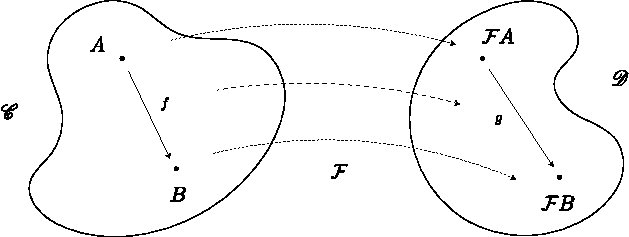
\includegraphics[scale=1]{fig/faith-full.pdf}
	\caption{For all $A, B$, and $g$, a faithful functor sends at \textit{most} one solid arrow in $\cat{C}$ to $g$. A full functor sends at \textit{least} one solid arrow in $\cat{C}$ to $g$.}
\end{figure}

\begin{ex}
The inclusion functor from $\cat{S}$ to $\cat{C}$ is always faithful, and it's full if and only if $\cat{S}$ is a full subcategory.
\end{ex}

\begin{defn}[]
The following definitions apply for a covariant functor $\mathcal{F}$ if, given any short exact $0\to A\to B\to C\to 0$, the given induced sequences are also exact.
\begin{equation*}
        \begin{aligned}[c]
                \text{\textbf{exact}} \\
                \text{\textbf{left exact}} \\
                \text{\textbf{right exact}}
        \end{aligned}
        \qquad
        \begin{aligned}[c]
                0\to \mathcal{F}A\to &\mathcal{F}B\to \mathcal{F}C\to 0\\
                0\to \mathcal{F}A\to &\mathcal{F}B\to \mathcal{F}C\\
                \mathcal{F}A\to &\mathcal{F}B\to \mathcal{F}C\to 0
        \end{aligned}
\end{equation*}
There are similar definitions for a contravariant functor $\mathcal{G}$.
\begin{equation*}
        \begin{aligned}[c]
                \text{\textbf{exact}} \\
                \text{\textbf{left exact}} \\
                \text{\textbf{right exact}}
        \end{aligned}
        \qquad
        \begin{aligned}[c]
                0\to \mathcal{G}C\to &\mathcal{G}B\to \mathcal{G}A\to 0\\
                0\to \mathcal{G}C\to &\mathcal{G}B\to \mathcal{G}A\\
                \mathcal{G}C\to &\mathcal{G}B\to \mathcal{G}A\to 0
        \end{aligned}
\end{equation*}
\end{defn}

%%%%%%%%%%%%%%%%%%%%
% Natural Transformations
%%%%%%%%%%%%%%%%%%%%

\section{Natural Transformations}

Natural transformations change one functor into another in a way that respects the underlying structure of the categories involved. It's kinda like a homotopy between $\mathcal{F}$ and $\mathcal{G}$ in the sense that for all $C \in \cat{C}$, it gives a morphism from $\mathcal{F}C$ to $\mathcal{G}C$.
\begin{figure}[H]
	\centering
	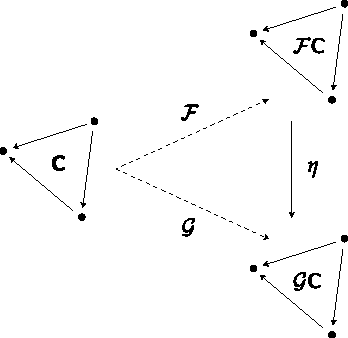
\includegraphics[scale=1]{fig/nat-trans.pdf}
\end{figure}

\begin{defn}
Suppose $\mathcal{F},\mathcal{G}:\cat{C}\to \cat{D}$ are functors. Then a \textbf{natural transformation} $\alpha:\mathcal{F}\Rightarrow \mathcal{G}$ is a family of \textbf{components}
\[
	\{ \eta_X: \mathcal{F}X \to \mathcal{G}X\}_X
\] such that the following diagram commutes for any $f:X\to Y$ in $\cat{C}$.
\[
\begin{tikzcd}
	\mathcal{F}X \rar{\eta_{X}} \arrow[d, "\mathcal{F}f"'] & \mathcal{G}X \dar{\mathcal{G}f} \\
	\mathcal{F}Y \rar{\eta_{Y}} & \mathcal{G}Y
\end{tikzcd}
\] 
\end{defn}
If every $\eta_{X}$ is an isomorphism, then $\eta$ is a \textbf{natural isomorphism} and we write $\eta: \mathcal{F} \cong \mathcal{G}$.


%+-------------------+
%| +---------------+ |
%| |    Chapter    | |
%| +---------------+ |
%+-------------------+
% Universal Properties

\chapter{Universal Properties}

%--------------------------------------------------------------------------------
% Common Examples
%--------------------------------------------------------------------------------
\section{Common Examples}

\begin{defn}[]
$(X, \left\{ \pi_{\alpha} \right\}_{\alpha})$ is a \textbf{product} of $\left\{ X_{\alpha} \right\}_{\alpha}$ if for all $Y$ and morphisms $f_{\alpha}:Y\to X_{\alpha}$, there is a unique morphism $f:Y\to X$ lifting each $f_{\alpha}$.
\[
\begin{tikzcd}
	& X\dar{\pi_{\alpha}} \\
	Y \arrow[ur,dashed,"\exists!\;f"]\rar["f_{\alpha}"'] & X_{\alpha}
\end{tikzcd}
\] 
\end{defn}

\begin{defn}[]
	$(X,  \left\{ \pi_{\alpha} \right\}_{\alpha})$ is a \textbf{coproduct} of $\left\{ X_{\alpha} \right\}_{\alpha}$ if for all $Y$ and morphisms $f_{\alpha}:X_{\alpha}\to Y$, there is a unique morphism $f:X\to Y$ extending each $f_{\alpha}$.
	\[
	\begin{tikzcd}
		& X\arrow[dl,dashed,"\exists!\;f"'] \\
		Y & X_{\alpha}\lar{f_{\alpha}}\uar["i_{\alpha}"']
	\end{tikzcd}
	\] 
\end{defn}

\begin{prop}
	If $(X,\left\{ \pi_{\alpha} \right\})$ is a product, then each $\pi_{\alpha}$ is epic. If $(X,\left\{ i_{\alpha} \right\})$ is a coproduct, then each $i_{\alpha}$ is monic.
\end{prop}

\begin{defn}[]
	$(F, i)$ is free on the set $B$ if for all objects $X$ and maps $f:B\to X$, there is a unique morphism $F\to X$ extending $f$.
	\[
	\begin{tikzcd}
		F \arrow[dr,dashed,"\exists!"] \\
		B \uar{i}\rar["f"'] & X
	\end{tikzcd}
	\] 
\end{defn}


\end{document}
